\section{Modelagem de Dados}
\label{sec:4.4}

A modelagem de dados do IGRIS foi projetada com foco na integridade referencial e na otimização de consultas, utilizando o Sistema Gerenciador de Banco de Dados relacional PostgreSQL 15. Conforme \citeonline{silberschatz2001}, o modelo relacional oferece mecanismos robustos para garantir a integridade e a consistência dos dados, fundamentais para aplicações críticas que envolvem múltiplos módulos interdependentes.

\subsection{Diagrama Entidade-Relacionamento}
\label{subsec:4.4.1}

Devido à complexidade do domínio e ao número de tabelas envolvidas, o modelo de dados é apresentado em quatro perspectivas complementares: uma visão geral consolidada e três recortes temáticos.

A Figura do DER Completo apresenta uma visão panorâmica de todas as tabelas e seus relacionamentos, permitindo compreender a estrutura global do banco de dados.

O módulo acadêmico abrange as entidades centrais do negócio: curso, turma, disciplina, disciplina\_curso, matriz, usuario\_disciplina, coordenador\_curso\_instituicao, dia\_semana, turno, disponibilidade, alocacao\_grade e grade. A entidade alocacao\_grade é o coração do sistema, registrando cada alocação gerada pelo algoritmo genético ao vincular uma matriz, uma disponibilidade e uma grade.

O módulo de controle de acesso consolida as entidades responsáveis pela segurança e autenticação: usuario, perfil, usuario\_perfil, link, tipo\_link, coordenacao, coordenacao\_vinculo, feedback e categorias\_feedback. A tabela usuario\_perfil implementa o controle multi-perfil, permitindo que um mesmo usuário assuma diferentes papéis institucionais.

O módulo institucional representa a configuração das instituições: instituicao, config\_faculdade, instituicao\_config, config\_sistema e erros. Essas entidades permitem que cada instituição personalize seus parâmetros operacionais de forma independente, incluindo os hiperparâmetros do algoritmo genético armazenados em config\_sistema.

\begin{landscape}

\begin{figure}[H]
\centering
\caption{Diagrama de Entidade-Relacionamento: Módulo de Controle de Acesso}
\label{fig:der_acesso}
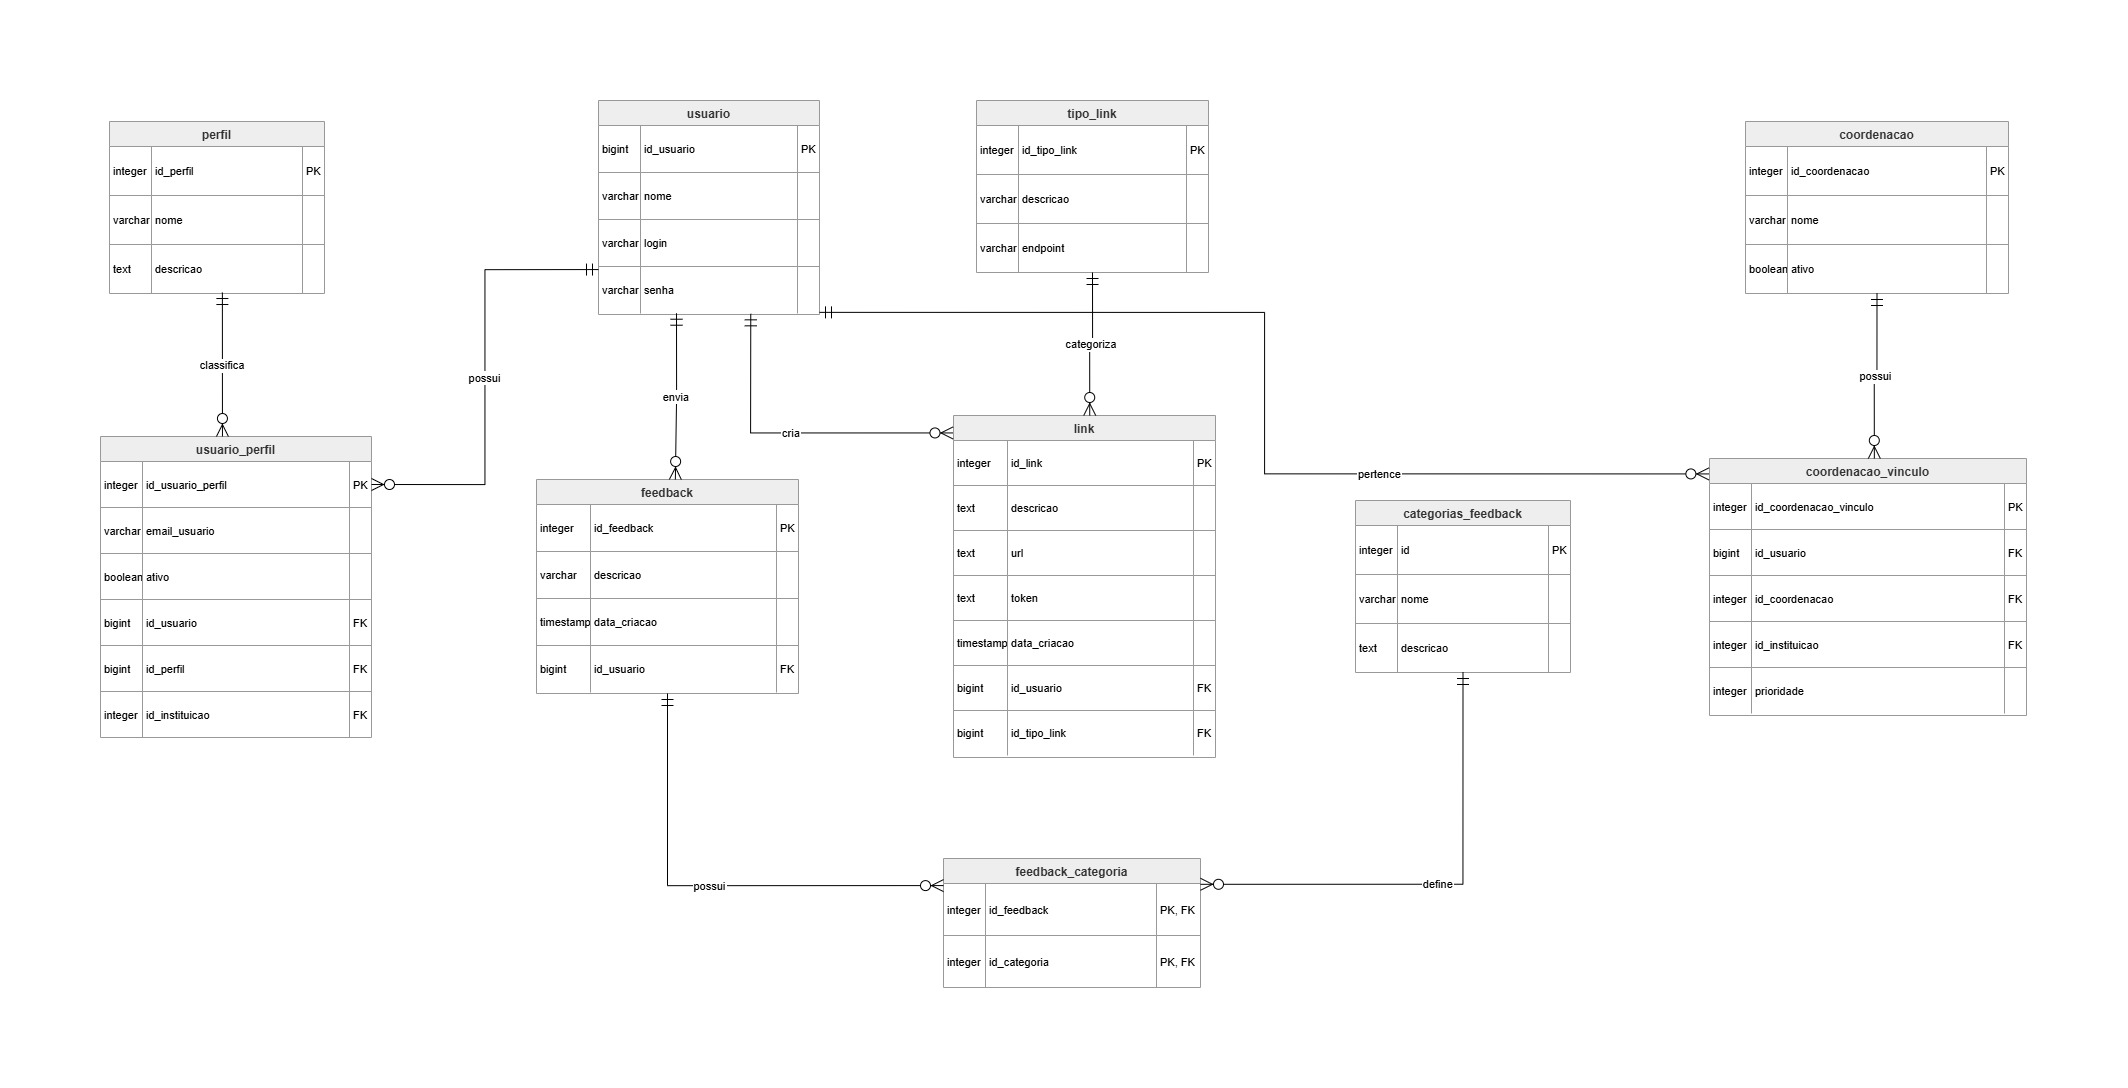
\includegraphics[width=\linewidth,height=0.9\textheight,keepaspectratio]{figuras/Figura_11_Diagrama ER_controle de acesso.jpg}
\fonteautores
\end{figure}

\newpage

\begin{figure}[H]
\centering
\caption{Diagrama de Entidade-Relacionamento: Módulo Acadêmico}
\label{fig:der_academico}
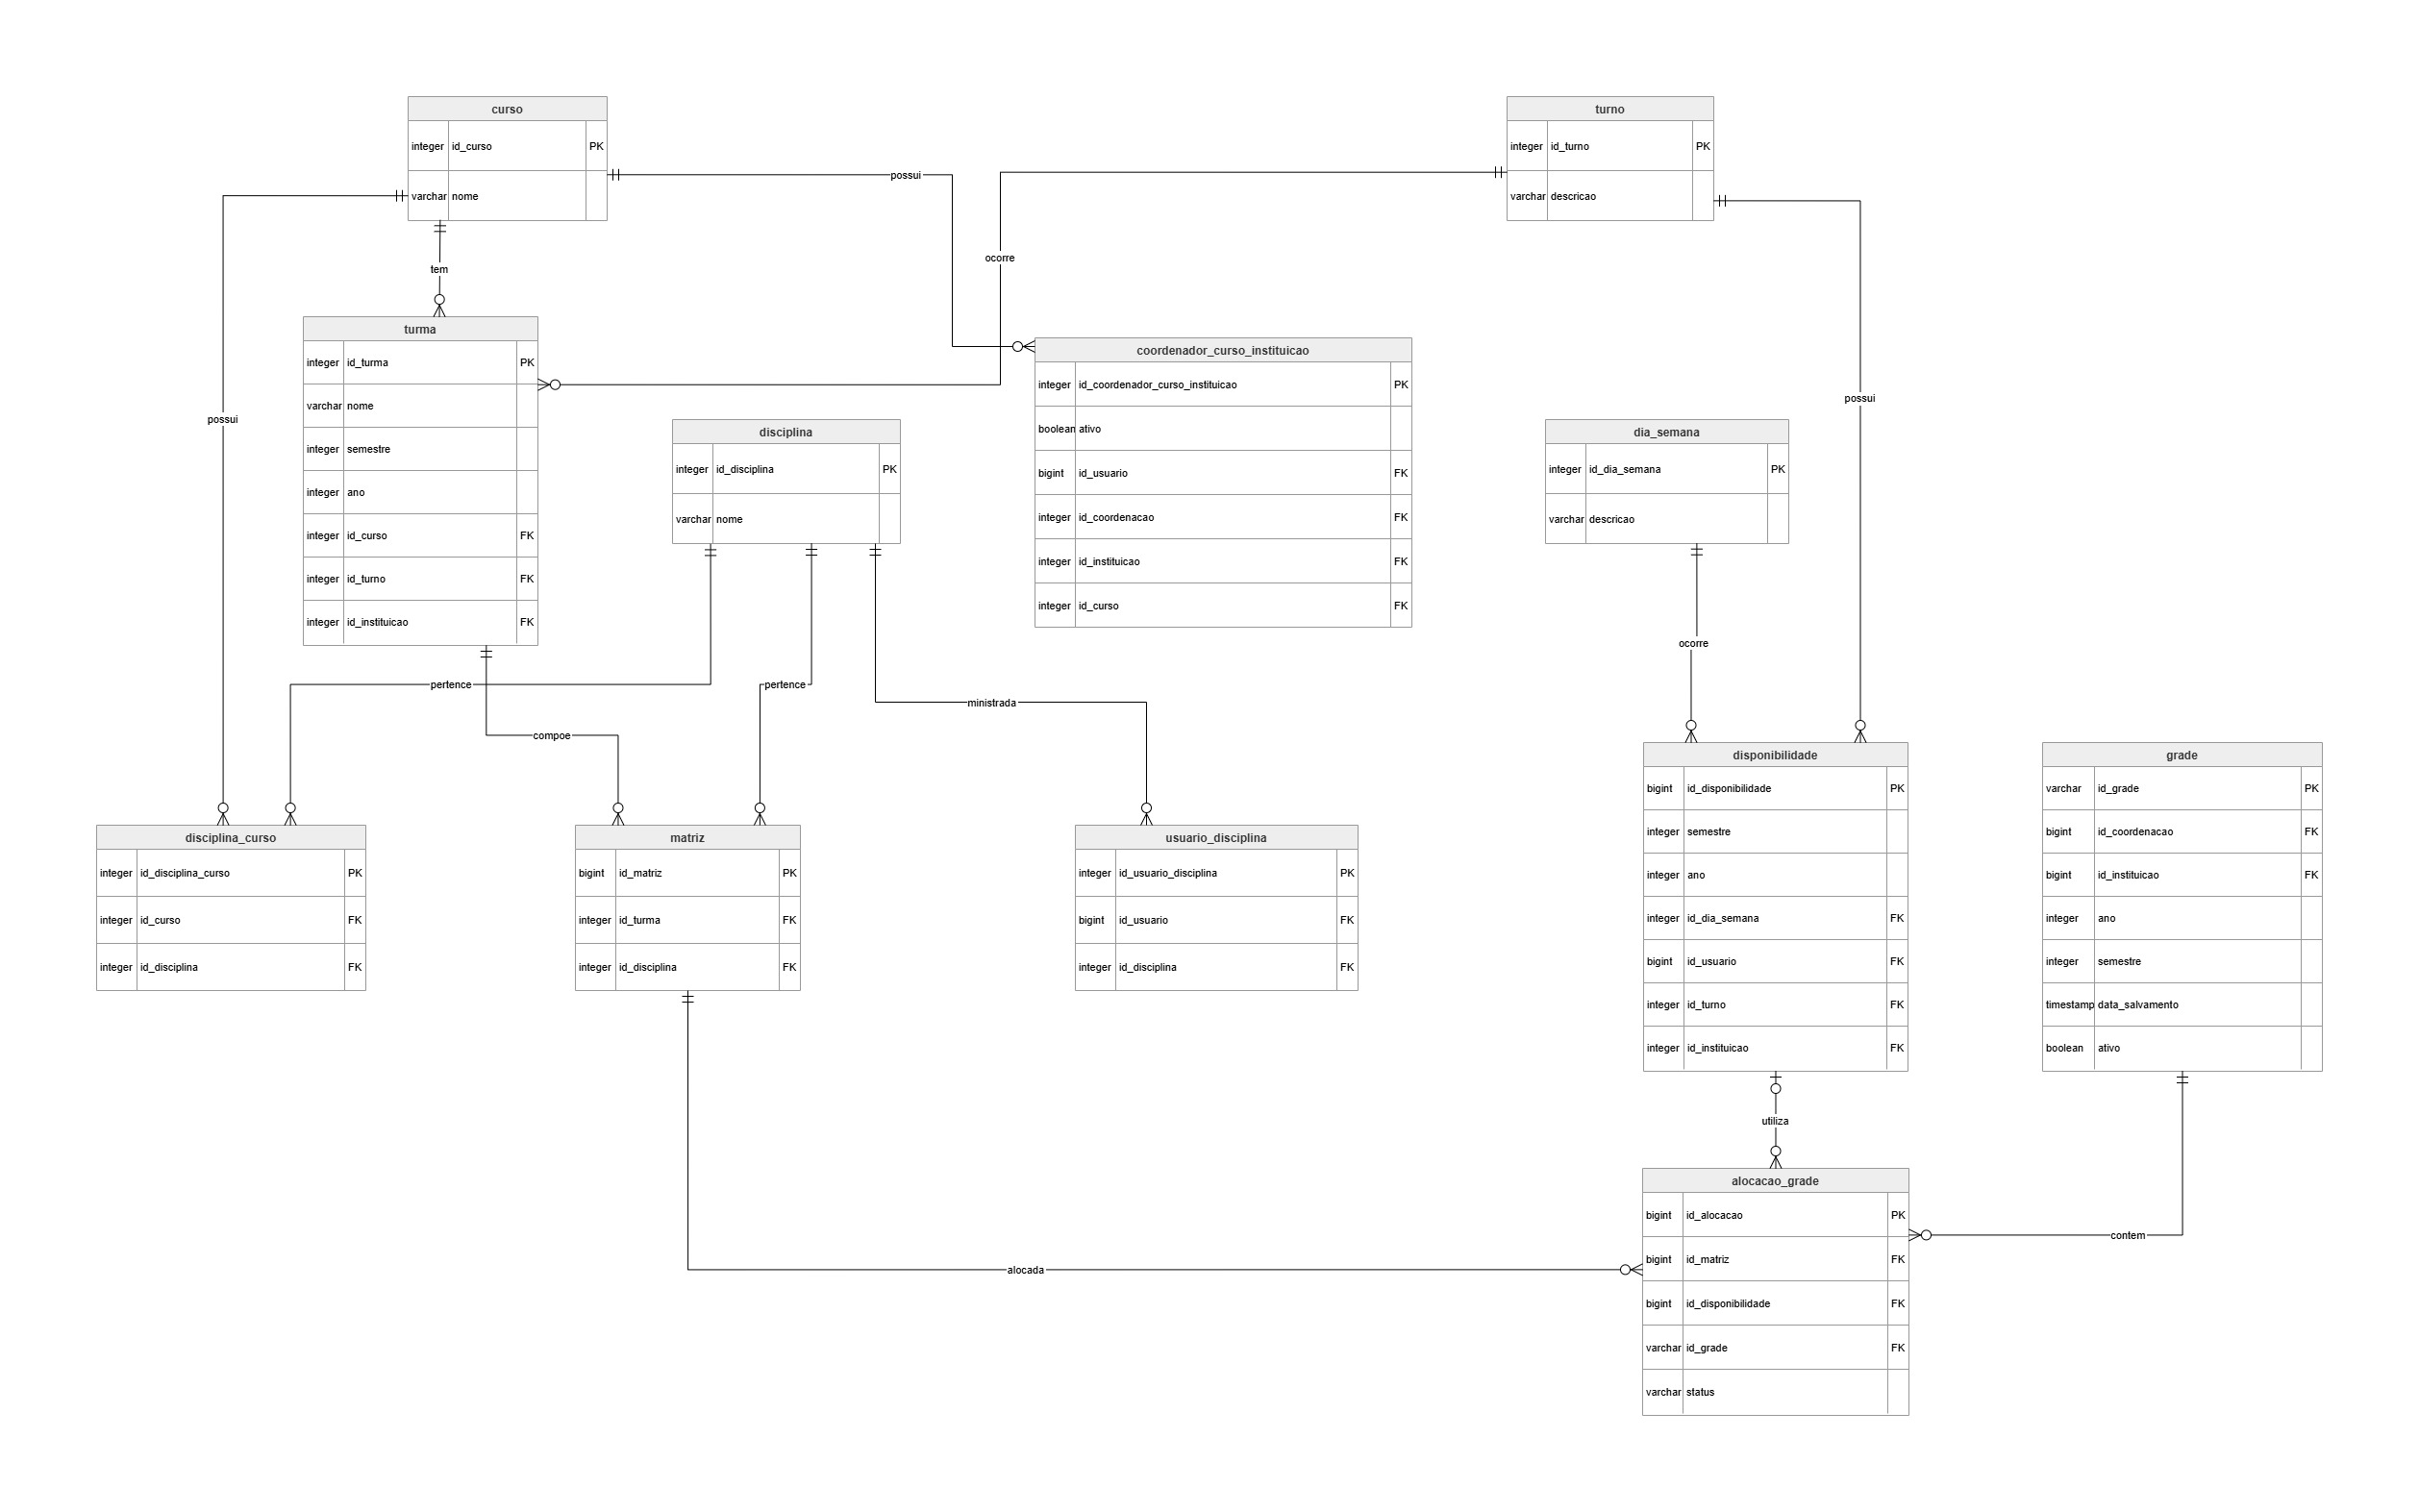
\includegraphics[width=\linewidth,height=0.9\textheight,keepaspectratio]{figuras/Figura_12_diagrama ER_academico.jpg}
\fonteautores
\end{figure}

\newpage

\begin{figure}[H]
\centering
\caption{Diagrama de Entidade-Relacionamento: Módulo Institucional}
\label{fig:der_institucional}
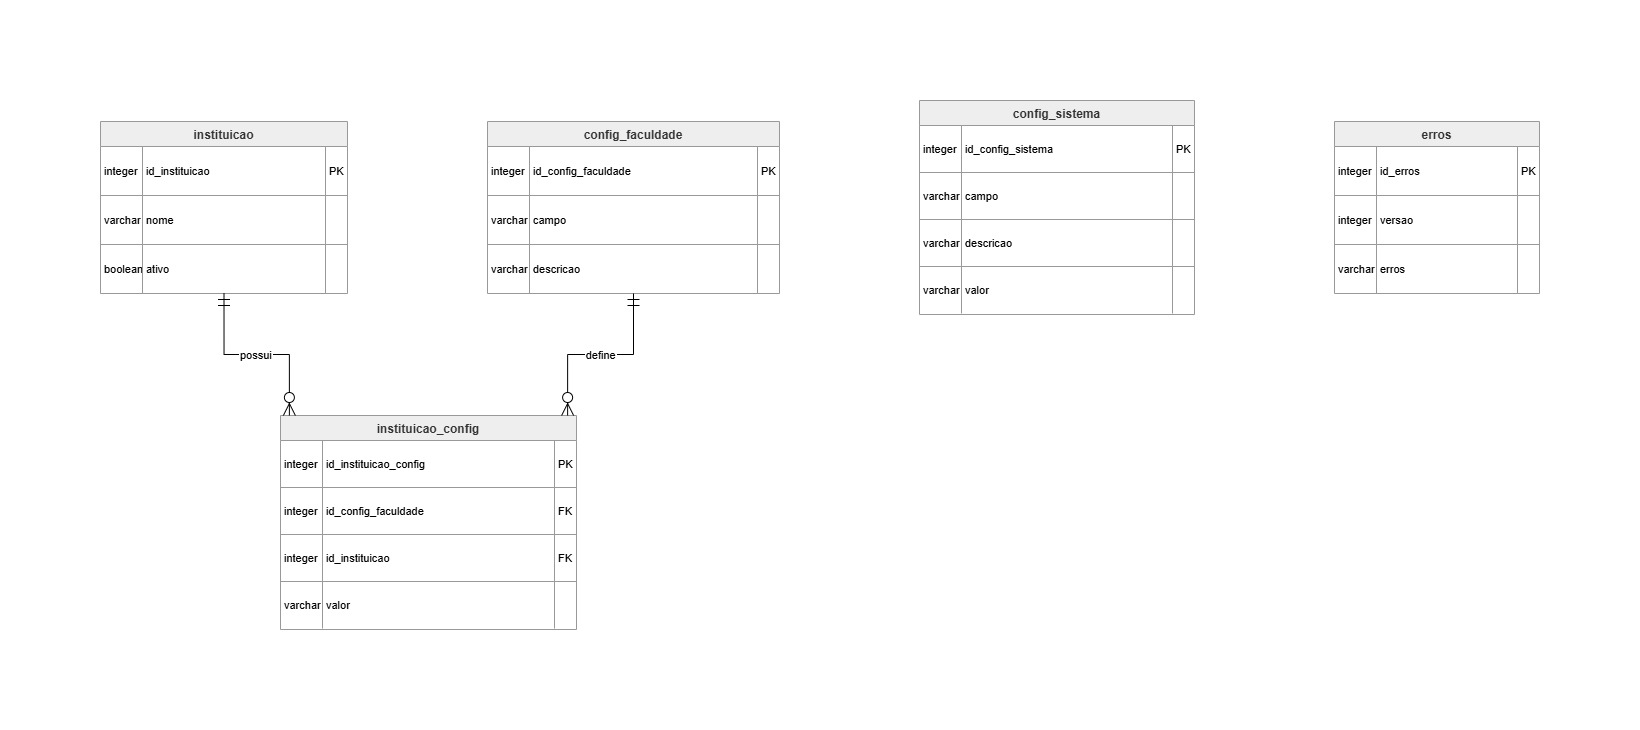
\includegraphics[width=\linewidth,height=0.9\textheight,keepaspectratio]{figuras/Figura_13_diagrama ER instituicao.jpg}
\fonteautores
\end{figure}

\end{landscape}

\begin{landscape}

\begin{figure}[H]
\centering
\caption{Diagrama de Entidade-Relacionamento Completo}
\label{fig:der_completo}
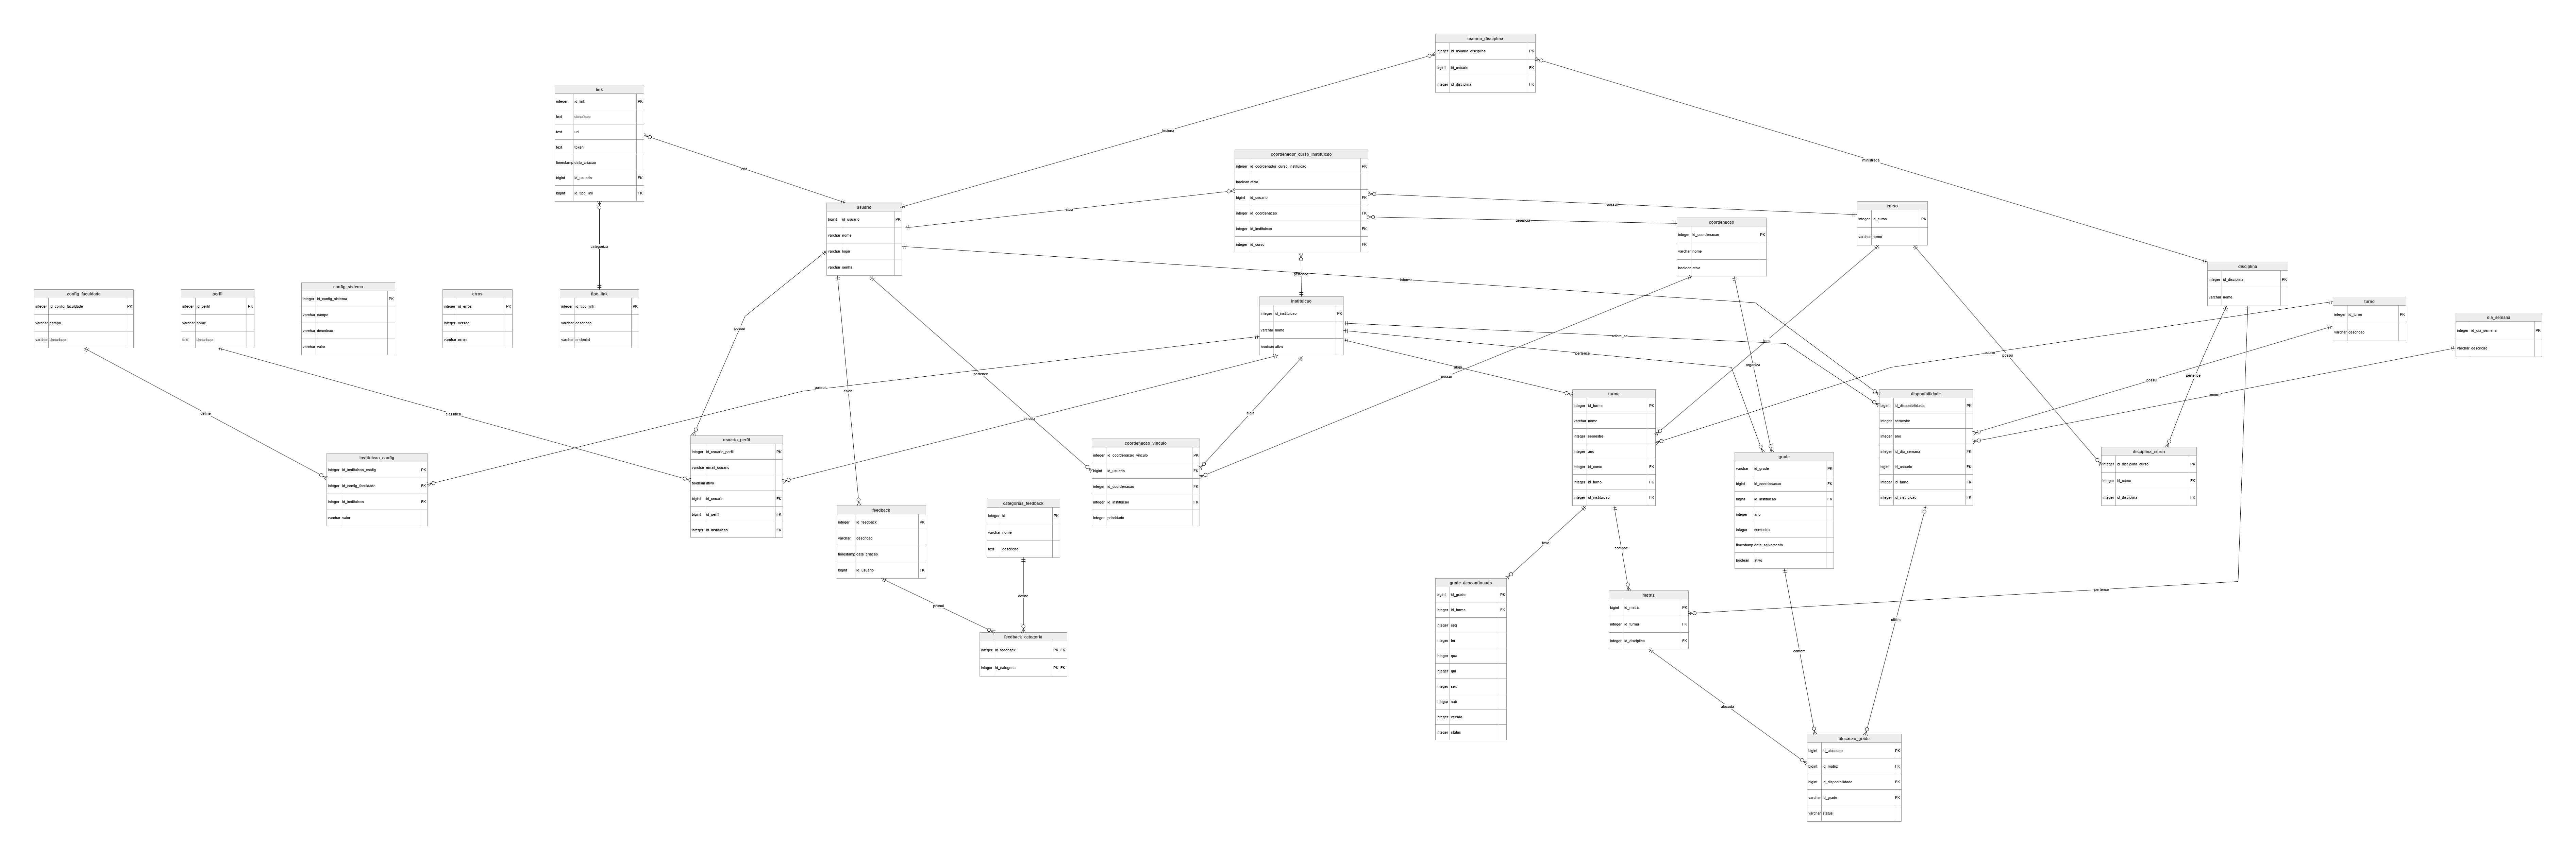
\includegraphics[width=\linewidth,height=\textheight,keepaspectratio]{figuras/Figura_14_diagrama ER completo.jpg}
\fonteautores
\end{figure}

\end{landscape}

\subsection{Dicionário de Dados}
\label{subsec:4.4.2}

\begingroup
\small
\sloppy
\setlength{\tabcolsep}{3pt}

O dicionário de dados complementa a representação gráfica do Modelo Entidade-Relacionamento, descrevendo a estrutura física das tabelas com tipos de dados, restrições de integridade e a semântica de cada atributo. Os Quadros de Tabela 37 a Tabela 63 apresentam a especificação completa das 27 tabelas do banco de dados do IGRIS.

% Tabela 37
\vspace{\baselineskip}

\Needspace{0.32\textheight}
\begin{longtable}{|L{5.2cm}|L{3.2cm}|L{2.4cm}|L{3.4cm}|}
\caption{instituicao} \\
\hline
\textbf{Variável} & \textbf{Tipo} & \textbf{Propriedades} & \textbf{Descrição} \\
\hline
\endfirsthead
\hline
\textbf{Variável} & \textbf{Tipo} & \textbf{Propriedades} & \textbf{Descrição} \\
\hline
\endhead
id\_instituicao & Integer (4 bytes) & PK & Código de identificação da tabela \\
\hline
nome & character varying (255) & NOT NULL & Nome da instituição de ensino \\
\hline
ativo & boolean (1 byte) & NOT NULL & Indica se a instituição está ativa no sistema \\
\hline
\end{longtable}

\fonteautores

% Tabela 38
\vspace{\baselineskip}

\Needspace{0.32\textheight}
\begin{longtable}{|L{5.2cm}|L{3.2cm}|L{2.4cm}|L{3.4cm}|}
\caption{config\_faculdade} \\
\hline
\textbf{Variável} & \textbf{Tipo} & \textbf{Propriedades} & \textbf{Descrição} \\
\hline
\endfirsthead
\hline
\textbf{Variável} & \textbf{Tipo} & \textbf{Propriedades} & \textbf{Descrição} \\
\hline
\endhead
id\_config\_faculdade & Integer (4 bytes) & PK & Código de identificação da tabela \\
\hline
campo & character varying (255) & NOT NULL & Nome identificador da configuração \\
\hline
descricao & character varying (255) & NULL & Descrição textual explicando a finalidade da configuração \\
\hline
\end{longtable}

\fonteautores

% Tabela 39
\vspace{\baselineskip}

\Needspace{0.32\textheight}
\begin{longtable}{|L{5.2cm}|L{3.2cm}|L{2.4cm}|L{3.4cm}|}
\caption{instituicao\_config} \\
\hline
\textbf{Variável} & \textbf{Tipo} & \textbf{Propriedades} & \textbf{Descrição} \\
\hline
\endfirsthead
\hline
\textbf{Variável} & \textbf{Tipo} & \textbf{Propriedades} & \textbf{Descrição} \\
\hline
\endhead
id\_instituicao\_config & Integer (4 bytes) & PK & Código de identificação da tabela \\
\hline
id\_config\_faculdade & Integer (4 bytes) & FK – config\_faculdade & Referência à configuração do catálogo \\
\hline
id\_instituicao & Integer (4 bytes) & FK – instituicao & Referência à instituição dona da configuração \\
\hline
valor & character varying (255) & NULL & Valor atribuído à configuração para esta instituição \\
\hline
\end{longtable}

\fonteautores

% Tabela 40
\vspace{\baselineskip}

\Needspace{0.32\textheight}
\begin{longtable}{|L{5.2cm}|L{3.2cm}|L{2.4cm}|L{3.4cm}|}
\caption{config\_sistema} \\
\hline
\textbf{Variável} & \textbf{Tipo} & \textbf{Propriedades} & \textbf{Descrição} \\
\hline
\endfirsthead
\hline
\textbf{Variável} & \textbf{Tipo} & \textbf{Propriedades} & \textbf{Descrição} \\
\hline
\endhead
id\_config\_sistema & Integer (4 bytes) & PK & Código de identificação da tabela \\
\hline
campo & character varying (255) & NOT NULL & Nome identificador do parâmetro (ex: TAMANHO\_POPULACAO) \\
\hline
descricao & character varying (255) & NULL & Descrição textual explicando o parâmetro \\
\hline
valor & character varying (255) & NULL & Valor atual do parâmetro \\
\hline
\end{longtable}

\fonteautores

% Tabela 41
\vspace{\baselineskip}

\Needspace{0.32\textheight}
\begin{longtable}{|L{5.2cm}|L{3.2cm}|L{2.4cm}|L{3.4cm}|}
\caption{erros} \\
\hline
\textbf{Variável} & \textbf{Tipo} & \textbf{Propriedades} & \textbf{Descrição} \\
\hline
\endfirsthead
\hline
\textbf{Variável} & \textbf{Tipo} & \textbf{Propriedades} & \textbf{Descrição} \\
\hline
\endhead
id\_erros & Integer (4 bytes) & PK & Código de identificação da tabela \\
\hline
versao & Integer (4 bytes) & NULL & Número da versão do sistema no momento do erro \\
\hline
erros & character varying (255) & NULL & Descrição textual do erro registrado \\
\hline
\end{longtable}

\fonteautores

% Tabela 42
\vspace{\baselineskip}

\Needspace{0.32\textheight}
\begin{longtable}{|L{5.2cm}|L{3.2cm}|L{2.4cm}|L{3.4cm}|}
\caption{usuario} \\
\hline
\textbf{Variável} & \textbf{Tipo} & \textbf{Propriedades} & \textbf{Descrição} \\
\hline
\endfirsthead
\hline
\textbf{Variável} & \textbf{Tipo} & \textbf{Propriedades} & \textbf{Descrição} \\
\hline
\endhead
id\_usuario & bigint (8 bytes) & PK & Código de identificação da tabela \\
\hline
nome & character varying (255) & NOT NULL & Nome completo do usuário \\
\hline
login & character varying (255) & NOT NULL, UNIQUE & Login único de acesso ao sistema \\
\hline
senha & character varying (255) & NOT NULL & Senha criptografada (BCrypt) do usuário \\
\hline
\end{longtable}

\fonteautores

% Tabela 43
\vspace{\baselineskip}

\Needspace{0.32\textheight}
\begin{longtable}{|L{5.2cm}|L{3.2cm}|L{2.4cm}|L{3.4cm}|}
\caption{perfil} \\
\hline
\textbf{Variável} & \textbf{Tipo} & \textbf{Propriedades} & \textbf{Descrição} \\
\hline
\endfirsthead
\hline
\textbf{Variável} & \textbf{Tipo} & \textbf{Propriedades} & \textbf{Descrição} \\
\hline
\endhead
id\_perfil & Integer (4 bytes) & PK & Código de identificação da tabela \\
\hline
nome & character varying (255) & NOT NULL & Nome do perfil de acesso \\
\hline
descricao & text (variável) & NULL & Descrição das permissões do perfil \\
\hline
\end{longtable}

\fonteautores

% Tabela 44
\vspace{\baselineskip}

\Needspace{0.32\textheight}
\begin{longtable}{|L{5.2cm}|L{3.2cm}|L{2.4cm}|L{3.4cm}|}
\caption{usuario\_perfil} \\
\hline
\textbf{Variável} & \textbf{Tipo} & \textbf{Propriedades} & \textbf{Descrição} \\
\hline
\endfirsthead
\hline
\textbf{Variável} & \textbf{Tipo} & \textbf{Propriedades} & \textbf{Descrição} \\
\hline
\endhead
id\_usuario\_perfil & Integer (4 bytes) & PK & Código de identificação da tabela \\
\hline
email\_usuario & character varying (255) & NULL & E-mail do usuário neste vínculo específico \\
\hline
ativo & boolean (1 byte) & NOT NULL & Indica se este vínculo de perfil está ativo \\
\hline
id\_usuario & bigint (8 bytes) & FK – usuario & Referência ao usuário \\
\hline
id\_perfil & bigint (8 bytes) & FK – perfil & Referência ao perfil de acesso \\
\hline
id\_instituicao & Integer (4 bytes) & FK – instituicao & Referência à instituição do vínculo \\
\hline
\end{longtable}

\fonteautores

% Tabela 45
\vspace{\baselineskip}

\Needspace{0.32\textheight}
\begin{longtable}{|L{5.2cm}|L{3.2cm}|L{2.4cm}|L{3.4cm}|}
\caption{tipo\_link} \\
\hline
\textbf{Variável} & \textbf{Tipo} & \textbf{Propriedades} & \textbf{Descrição} \\
\hline
\endfirsthead
\hline
\textbf{Variável} & \textbf{Tipo} & \textbf{Propriedades} & \textbf{Descrição} \\
\hline
\endhead
id\_tipo\_link & Integer (4 bytes) & PK & Código de identificação da tabela \\
\hline
descricao & character varying (255) & NOT NULL & Descrição do tipo de link \\
\hline
endpoint & character varying (255) & NULL & Rota/endpoint associado ao tipo de link \\
\hline
\end{longtable}

\fonteautores

% Tabela 46
\vspace{\baselineskip}

\Needspace{0.32\textheight}
\begin{longtable}{|L{5.2cm}|L{3.2cm}|L{2.4cm}|L{3.4cm}|}
\caption{link} \\
\hline
\textbf{Variável} & \textbf{Tipo} & \textbf{Propriedades} & \textbf{Descrição} \\
\hline
\endfirsthead
\hline
\textbf{Variável} & \textbf{Tipo} & \textbf{Propriedades} & \textbf{Descrição} \\
\hline
\endhead
id\_link & Integer (4 bytes) & PK & Código de identificação da tabela \\
\hline
descricao & text (variável) & NULL & Descrição ou finalidade do link gerado \\
\hline
url & text (variável) & NULL & URL completa do link gerado \\
\hline
token & text (variável) & NOT NULL & Token criptografado para validação do link \\
\hline
data\_criacao & timestamp (8 bytes) & NOT NULL & Data e hora da criação do link \\
\hline
id\_usuario & bigint (8 bytes) & FK – usuario & Referência ao usuário que criou o link \\
\hline
id\_tipo\_link & bigint (8 bytes) & FK – tipo\_link & Referência ao tipo de link \\
\hline
\end{longtable}

\fonteautores

% Tabela 47
\vspace{\baselineskip}

\Needspace{0.32\textheight}
\begin{longtable}{|L{5.2cm}|L{3.2cm}|L{2.4cm}|L{3.4cm}|}
\caption{feedback} \\
\hline
\textbf{Variável} & \textbf{Tipo} & \textbf{Propriedades} & \textbf{Descrição} \\
\hline
\endfirsthead
\hline
\textbf{Variável} & \textbf{Tipo} & \textbf{Propriedades} & \textbf{Descrição} \\
\hline
\endhead
id\_feedback & Integer (4 bytes) & PK & Código de identificação da tabela \\
\hline
descricao & character varying (255) & NOT NULL & Texto descritivo do feedback enviado \\
\hline
data\_criacao & timestamp (8 bytes) & NOT NULL & Data e hora do envio do feedback \\
\hline
id\_usuario & bigint (8 bytes) & FK – usuario & Referência ao usuário remetente \\
\hline
\end{longtable}

\fonteautores

% Tabela 48
\vspace{\baselineskip}

\Needspace{0.32\textheight}
\begin{longtable}{|L{5.2cm}|L{3.2cm}|L{2.4cm}|L{3.4cm}|}
\caption{categorias\_feedback} \\
\hline
\textbf{Variável} & \textbf{Tipo} & \textbf{Propriedades} & \textbf{Descrição} \\
\hline
\endfirsthead
\hline
\textbf{Variável} & \textbf{Tipo} & \textbf{Propriedades} & \textbf{Descrição} \\
\hline
\endhead
id & Integer (4 bytes) & PK & Código de identificação da tabela \\
\hline
nome & character varying (255) & NOT NULL & Nome da categoria \\
\hline
descricao & text (variável) & NULL & Descrição detalhada da categoria \\
\hline
\end{longtable}

\fonteautores

% Tabela 49
\vspace{\baselineskip}

\Needspace{0.32\textheight}
\begin{longtable}{|L{5.2cm}|L{3.2cm}|L{2.4cm}|L{3.4cm}|}
\caption{feedback\_categoria} \\
\hline
\textbf{Variável} & \textbf{Tipo} & \textbf{Propriedades} & \textbf{Descrição} \\
\hline
\endfirsthead
\hline
\textbf{Variável} & \textbf{Tipo} & \textbf{Propriedades} & \textbf{Descrição} \\
\hline
\endhead
id\_feedback & Integer (4 bytes) & PK, FK – feedback & Referência ao feedback \\
\hline
id\_categoria & Integer (4 bytes) & PK, FK – categorias\_feedback & Referência à categoria do feedback \\
\hline
\end{longtable}

\fonteautores

% Tabela 50
\vspace{\baselineskip}

\Needspace{0.32\textheight}
\begin{longtable}{|L{5.2cm}|L{3.2cm}|L{2.4cm}|L{3.4cm}|}
\caption{coordenacao} \\
\hline
\textbf{Variável} & \textbf{Tipo} & \textbf{Propriedades} & \textbf{Descrição} \\
\hline
\endfirsthead
\hline
\textbf{Variável} & \textbf{Tipo} & \textbf{Propriedades} & \textbf{Descrição} \\
\hline
\endhead
id\_coordenacao & Integer (4 bytes) & PK & Código de identificação da tabela \\
\hline
nome & character varying (255) & NOT NULL & Nome da coordenação/departamento \\
\hline
ativo & boolean (1 byte) & NOT NULL & Indica se a coordenação está ativa \\
\hline
\end{longtable}

\fonteautores

% Tabela 51
\vspace{\baselineskip}

\Needspace{0.32\textheight}
\begin{longtable}{|L{5.2cm}|L{3.2cm}|L{2.4cm}|L{3.4cm}|}
\caption{coordenacao\_vinculo} \\
\hline
\textbf{Variável} & \textbf{Tipo} & \textbf{Propriedades} & \textbf{Descrição} \\
\hline
\endfirsthead
\hline
\textbf{Variável} & \textbf{Tipo} & \textbf{Propriedades} & \textbf{Descrição} \\
\hline
\endhead
id\_coordenacao\_vinculo & Integer (4 bytes) & PK & Código de identificação da tabela \\
\hline
id\_usuario & bigint (8 bytes) & FK – usuario & Referência ao usuário (coordenador) \\
\hline
id\_coordenacao & Integer (4 bytes) & FK – coordenacao & Referência à coordenação \\
\hline
id\_instituicao & Integer (4 bytes) & FK – instituicao & Referência à instituição \\
\hline
prioridade & Integer (4 bytes) & NULL & Nível de prioridade do vínculo \\
\hline
\end{longtable}

\fonteautores

% Tabela 52
\vspace{\baselineskip}

\Needspace{0.32\textheight}
\begin{longtable}{|L{5.2cm}|L{3.2cm}|L{2.4cm}|L{3.4cm}|}
\caption{curso} \\
\hline
\textbf{Variável} & \textbf{Tipo} & \textbf{Propriedades} & \textbf{Descrição} \\
\hline
\endfirsthead
\hline
\textbf{Variável} & \textbf{Tipo} & \textbf{Propriedades} & \textbf{Descrição} \\
\hline
\endhead
id\_curso & Integer (4 bytes) & PK & Código de identificação da tabela \\
\hline
nome & character varying (255) & NOT NULL & Nome do curso \\
\hline
\end{longtable}

\fonteautores

% Tabela 53
\vspace{\baselineskip}

\Needspace{0.32\textheight}
\begin{longtable}{|L{5.2cm}|L{3.2cm}|L{2.4cm}|L{3.4cm}|}
\caption{turno} \\
\hline
\textbf{Variável} & \textbf{Tipo} & \textbf{Propriedades} & \textbf{Descrição} \\
\hline
\endfirsthead
\hline
\textbf{Variável} & \textbf{Tipo} & \textbf{Propriedades} & \textbf{Descrição} \\
\hline
\endhead
id\_turno & Integer (4 bytes) & PK & Código de identificação da tabela \\
\hline
descricao & character varying (50) & NOT NULL & Nome/descrição do turno \\
\hline
\end{longtable}

\fonteautores

% Tabela 54
\vspace{\baselineskip}

\Needspace{0.32\textheight}
\begin{longtable}{|L{5.2cm}|L{3.2cm}|L{2.4cm}|L{3.4cm}|}
\caption{dia\_semana} \\
\hline
\textbf{Variável} & \textbf{Tipo} & \textbf{Propriedades} & \textbf{Descrição} \\
\hline
\endfirsthead
\hline
\textbf{Variável} & \textbf{Tipo} & \textbf{Propriedades} & \textbf{Descrição} \\
\hline
\endhead
id\_dia\_semana & Integer (4 bytes) & PK & Código de identificação da tabela \\
\hline
descricao & character varying (50) & NOT NULL & Nome do dia da semana \\
\hline
\end{longtable}

\fonteautores

% Tabela 55
\vspace{\baselineskip}

\Needspace{0.32\textheight}
\begin{longtable}{|L{5.2cm}|L{3.2cm}|L{2.4cm}|L{3.4cm}|}
\caption{disciplina} \\
\hline
\textbf{Variável} & \textbf{Tipo} & \textbf{Propriedades} & \textbf{Descrição} \\
\hline
\endfirsthead
\hline
\textbf{Variável} & \textbf{Tipo} & \textbf{Propriedades} & \textbf{Descrição} \\
\hline
\endhead
id\_disciplina & Integer (4 bytes) & PK & Código de identificação da tabela \\
\hline
nome & character varying (255) & NOT NULL & Nome da disciplina \\
\hline
\end{longtable}

\fonteautores

% Tabela 56
\vspace{\baselineskip}

\Needspace{0.32\textheight}
\begin{longtable}{|L{5.2cm}|L{3.2cm}|L{2.4cm}|L{3.4cm}|}
\caption{turma} \\
\hline
\textbf{Variável} & \textbf{Tipo} & \textbf{Propriedades} & \textbf{Descrição} \\
\hline
\endfirsthead
\hline
\textbf{Variável} & \textbf{Tipo} & \textbf{Propriedades} & \textbf{Descrição} \\
\hline
\endhead
id\_turma & Integer (4 bytes) & PK & Código de identificação da tabela \\
\hline
nome & character varying (255) & NOT NULL & Nome ou identificador da turma \\
\hline
semestre & Integer (4 bytes) & NOT NULL & Semestre letivo da turma (1 ou 2) \\
\hline
ano & Integer (4 bytes) & NOT NULL & Ano letivo da turma \\
\hline
id\_curso & Integer (4 bytes) & FK – curso & Referência ao curso da turma \\
\hline
id\_turno & Integer (4 bytes) & FK – turno & Referência ao turno da turma \\
\hline
id\_instituicao & Integer (4 bytes) & FK – instituicao & Referência à instituição da turma \\
\hline
\end{longtable}

\fonteautores

% Tabela 57
\vspace{\baselineskip}

\Needspace{0.32\textheight}
\begin{longtable}{|L{5.2cm}|L{3.2cm}|L{2.4cm}|L{3.4cm}|}
\caption{disciplina\_curso} \\
\hline
\textbf{Variável} & \textbf{Tipo} & \textbf{Propriedades} & \textbf{Descrição} \\
\hline
\endfirsthead
\hline
\textbf{Variável} & \textbf{Tipo} & \textbf{Propriedades} & \textbf{Descrição} \\
\hline
\endhead
id\_disciplina\_curso & Integer (4 bytes) & PK & Código de identificação da tabela \\
\hline
id\_curso & Integer (4 bytes) & FK – curso & Referência ao curso \\
\hline
id\_disciplina & Integer (4 bytes) & FK – disciplina & Referência à disciplina \\
\hline
\end{longtable}

\fonteautores

% Tabela 58
\vspace{\baselineskip}

\Needspace{0.32\textheight}
\begin{longtable}{|L{5.2cm}|L{3.2cm}|L{2.4cm}|L{3.4cm}|}
\caption{matriz} \\
\hline
\textbf{Variável} & \textbf{Tipo} & \textbf{Propriedades} & \textbf{Descrição} \\
\hline
\endfirsthead
\hline
\textbf{Variável} & \textbf{Tipo} & \textbf{Propriedades} & \textbf{Descrição} \\
\hline
\endhead
id\_matriz & bigint (8 bytes) & PK & Código de identificação da tabela \\
\hline
id\_turma & Integer (4 bytes) & FK – turma & Referência à turma \\
\hline
id\_disciplina & Integer (4 bytes) & FK – disciplina & Referência à disciplina \\
\hline
\end{longtable}

\fonteautores

% Tabela 59
\vspace{\baselineskip}

\Needspace{0.32\textheight}
\begin{longtable}{|L{5.2cm}|L{3.2cm}|L{2.4cm}|L{3.4cm}|}
\caption{coordenador\_curso\_instituicao} \\
\hline
\textbf{Variável} & \textbf{Tipo} & \textbf{Propriedades} & \textbf{Descrição} \\
\hline
\endfirsthead
\hline
\textbf{Variável} & \textbf{Tipo} & \textbf{Propriedades} & \textbf{Descrição} \\
\hline
\endhead
id\_coordenador\_curso\_instituicao & Integer (4 bytes) & PK & Código de identificação da tabela \\
\hline
ativo & boolean (1 byte) & NOT NULL & Indica se o vínculo está ativo \\
\hline
id\_usuario & bigint (8 bytes) & FK – usuario & Referência ao usuário (coordenador) \\
\hline
id\_coordenacao & Integer (4 bytes) & FK – coordenacao & Referência à coordenação \\
\hline
id\_instituicao & Integer (4 bytes) & FK – instituicao & Referência à instituição \\
\hline
id\_curso & Integer (4 bytes) & FK – curso & Referência ao curso gerenciado \\
\hline
\end{longtable}

\fonteautores

% Tabela 60
\vspace{\baselineskip}

\Needspace{0.32\textheight}
\begin{longtable}{|L{5.2cm}|L{3.2cm}|L{2.4cm}|L{3.4cm}|}
\caption{usuario\_disciplina} \\
\hline
\textbf{Variável} & \textbf{Tipo} & \textbf{Propriedades} & \textbf{Descrição} \\
\hline
\endfirsthead
\hline
\textbf{Variável} & \textbf{Tipo} & \textbf{Propriedades} & \textbf{Descrição} \\
\hline
\endhead
id\_usuario\_disciplina & Integer (4 bytes) & PK & Código de identificação da tabela \\
\hline
id\_usuario & bigint (8 bytes) & FK – usuario & Referência ao usuário (professor) \\
\hline
id\_disciplina & Integer (4 bytes) & FK – disciplina & Referência à disciplina \\
\hline
\end{longtable}

\fonteautores

% Tabela 61
\vspace{\baselineskip}

\Needspace{0.32\textheight}
\begin{longtable}{|L{5.2cm}|L{3.2cm}|L{2.4cm}|L{3.4cm}|}
\caption{disponibilidade} \\
\hline
\textbf{Variável} & \textbf{Tipo} & \textbf{Propriedades} & \textbf{Descrição} \\
\hline
\endfirsthead
\hline
\textbf{Variável} & \textbf{Tipo} & \textbf{Propriedades} & \textbf{Descrição} \\
\hline
\endhead
id\_disponibilidade & bigint (8 bytes) & PK & Código de identificação da tabela \\
\hline
semestre & Integer (4 bytes) & NOT NULL & Semestre de referência da disponibilidade \\
\hline
ano & Integer (4 bytes) & NOT NULL & Ano de referência da disponibilidade \\
\hline
id\_dia\_semana & Integer (4 bytes) & FK – dia\_semana & Referência ao dia da semana disponível \\
\hline
id\_usuario & bigint (8 bytes) & FK – usuario & Referência ao usuário (professor) \\
\hline
id\_turno & Integer (4 bytes) & FK – turno & Referência ao turno disponível \\
\hline
id\_instituicao & Integer (4 bytes) & FK – instituicao & Referência à instituição do vínculo \\
\hline
\end{longtable}

\fonteautores

% Tabela 62
\vspace{\baselineskip}

\Needspace{0.32\textheight}
\begin{longtable}{|L{5.2cm}|L{3.2cm}|L{2.4cm}|L{3.4cm}|}
\caption{grade} \\
\hline
\textbf{Variável} & \textbf{Tipo} & \textbf{Propriedades} & \textbf{Descrição} \\
\hline
\endfirsthead
\hline
\textbf{Variável} & \textbf{Tipo} & \textbf{Propriedades} & \textbf{Descrição} \\
\hline
\endhead
id\_grade & character varying (36) & PK (UUID) & Código de identificação da tabela \\
\hline
id\_coordenacao & bigint (8 bytes) & FK – coordenacao & Referência à coordenação dona da grade \\
\hline
id\_instituicao & bigint (8 bytes) & FK – instituicao & Referência à instituição \\
\hline
ano & Integer (4 bytes) & NOT NULL & Ano letivo da grade \\
\hline
semestre & Integer (4 bytes) & NOT NULL & Semestre letivo da grade \\
\hline
data\_salvamento & timestamp (8 bytes) & NULL & Data e hora em que a grade foi salva \\
\hline
ativo & boolean (1 byte) & NOT NULL & Indica se a grade está ativa (em vigor) \\
\hline
\end{longtable}

\fonteautores

% Tabela 63
\vspace{\baselineskip}

\Needspace{0.32\textheight}
\begin{longtable}{|L{5.2cm}|L{3.2cm}|L{2.4cm}|L{3.4cm}|}
\caption{alocacao\_grade} \\
\hline
\textbf{Variável} & \textbf{Tipo} & \textbf{Propriedades} & \textbf{Descrição} \\
\hline
\endfirsthead
\hline
\textbf{Variável} & \textbf{Tipo} & \textbf{Propriedades} & \textbf{Descrição} \\
\hline
\endhead
id\_alocacao & bigint (8 bytes) & PK & Código de identificação da tabela \\
\hline
id\_matriz & bigint (8 bytes) & FK – matriz & Referência à matriz (turma + disciplina) \\
\hline
id\_disponibilidade & bigint (8 bytes) & FK – disponibilidade & Referência à disponibilidade (professor + dia + turno) \\
\hline
id\_grade & character varying (36) & FK – grade & Referência à grade à qual esta alocação pertence \\
\hline
status & character varying (50) & NULL & Status da alocação (ex: confirmada, pendente) \\
\hline
\end{longtable}

\fonteautores

\endgroup

% Chapter 6
